\documentclass[utf8x]{ctexart}
\usepackage{setspace}
\usepackage{url}
\onehalfspacing
\usepackage{amsmath,amssymb,amsfonts,amsthm,mathtools}
\usepackage[english]{babel}
\usepackage[T1]{fontenc}
\usepackage{lmodern}
\usepackage{dsfont}
\usepackage{bbm}
\usepackage[round]{natbib}
\usepackage{color} 
\usepackage[defaultlines=2,all]{nowidow}
\usepackage{caption}
\usepackage[labelformat=simple]{subcaption}
\usepackage{makecell}
\renewcommand\thesubfigure{(\alph{subfigure})}

\setlength\parindent{0pt}
\setlength{\parskip}{6pt plus 1pt minus 1pt}

\newcommand{\red}{\textcolor{red}}


\begin{document}

\begin{titlepage}
  \centering
  {\scshape\LARGE National Taiwan University \par}
  \vspace{1cm}
  {\scshape\Large Financial Technology \par}
  \vspace{2cm}
  {\huge\bfseries Project 1: Credit Card Fraud Detection\par}
  \vspace{2cm}
  {\Large Lecturer:\\
    Che Lin (林澤) \par}
  \vspace{1cm}
  {\Large Author: Tadeo Hepperle \par}
  \vfill
  {\large \today\par}
\end{titlepage}


\tableofcontents

\cleardoublepage

\section{Introduction}

In this project we use a dataset from Kaggle "Credit Card Fraud Detection" to predict fraudulent spendings on credit cards, given a range of features. For this task, we will compare classical machine learning models like logistic regression, support vector machines and random forests with deep neural networks and evaluate their performance.

\subsection{Description of the data}

The dataset was originally from Kaggle, named "Credit Card Fraud Detection" and contains 31 variables, grouped into 30 features and one class label. Two of these features are the time the transaction took place and the amount spent. The 28 remaining features were obtained by performing a principal component analysis on a larger dataset. The classlabel is either 0 (normal) or 1 (fraudulent) for each record. The entire data consists of 99999 independent transaction records. Of those only 223 are fraudulent, which amounts to only 0.22\% and makes the data extremely unbalanced.

\subsection{Description of methods}

Besides deep neural networks, we also take a brief look at logistic regression, support vector machines and random forest models.

\subsubsection{Logistic Regression}
In Logistic regression we try to predict a binary response by using an array of numeric features. The model formula looks like this:

\[ P(y=1) =  \frac{exp(\beta_0 + \beta_1x_1 + \dots + \beta_kx_k)}{1 + exp(\beta_0 + \beta_1x_1 + \dots + \beta_kx_k)}\]

where $P(y=1)$ represents the probability of class 1 (fraud in our case) and the $x_1, \dots, x_k$ represent $k$ predictors. The probability of the other class ($P(y=0)$) is therefore $1-P(y=1)$.
Because the derivative of the logistic function is never 0 there is no closed form solution and methods like gradient descent need to be used for optimization. However if the data is linearly separable, these methods will never converge and will result in an "infinitely steep" probability curve.

\subsubsection{Support Vector Machines}

Support Vector Machines (SVM) aim to find a hyperplane that linearly seperates the data linearly into 2 homogeneous halfspaces. Because this is not always possible, two tricks can be applied. First, it is useful to use a soft margin instead of a hard one which allows some points of the wrong class to lie in the half space of the other class as long as they are still pretty close to the hyperplane. In some cases, like noisy data this can even give better classification results in cases where a hard margin could perfectly seperate the two classes. The second "Trick" that can be used to make Support Vector machines more useful is to use a certain kernel function to transform the input features to a different space domain. This can make even originally not linearly seperable data, seperable if the right transformations are used. In this project, we will not experiment with any kernel functions.

\subsubsection{Random Forest Classifier}

Random Forest is an ensemble method. That means it combines the power of an array of weak learners that on their own would perform poorly. Typically decision trees are used as the weak classifier, hence the name random "Forest". There are multiple ideas, how to let the individual trees learn and how to combine them. in Bootstrapping for example, we let each tree learn on a bootstrapping sample of the original data and later take a majority vote among all trees as the final decision. The bootstrapping sample is produced by randomly sampling objects from the data n times with put backs (where $n$ is the number of objects in total). The sample is different for every tree and can therefore allow the trees to learn different aspects of the data. The problem with this approach is, that the bootstrapping samples are still highly correlated. Random Forest aims to solve this, by further diversifying and restricting what data can be used by each tree during learning. The idea is simple: At each split to be made in a decision tree, not all features are considered, but only a subset of features is allowed to be used to make the split. Typically for $k$ features, $\sqrt{k}$ randomly selected features are allowed in each split. This increases the variance among weak learners and can lead to classification improvements.

\section{Results}

With an 80-20 train-test split of the data, 3 models were trained: Logistic Regression, Support Vector Machine and Random Forest Classifier.

\subsection{Confusion Matrices and Classification Metrics}
As Figure~\ref{fig:confusion1} shows, all models are pretty good at classifying the non-fraud cases as non-fraud, which is non-surprising since these comprise the overwhelming majority of the training data.
Taking a look at the classification metrics in Table~\ref{tab:metrics1} we can see that the SVM is overall performing best, also with highest accuracy. To judge the performance, I would use the F1-score as it provides a good middle ground between precision and recall, in both of which high values are desired. I think the F1 metric is most suitable on this dataset because it is not so much affected by the very imbalanced distribution of fraud vs. non-fraud cases in the data.

\begin{figure}[htb]
  \centering
  \begin{subfigure}[b]{0.32\textwidth}
    \centering
    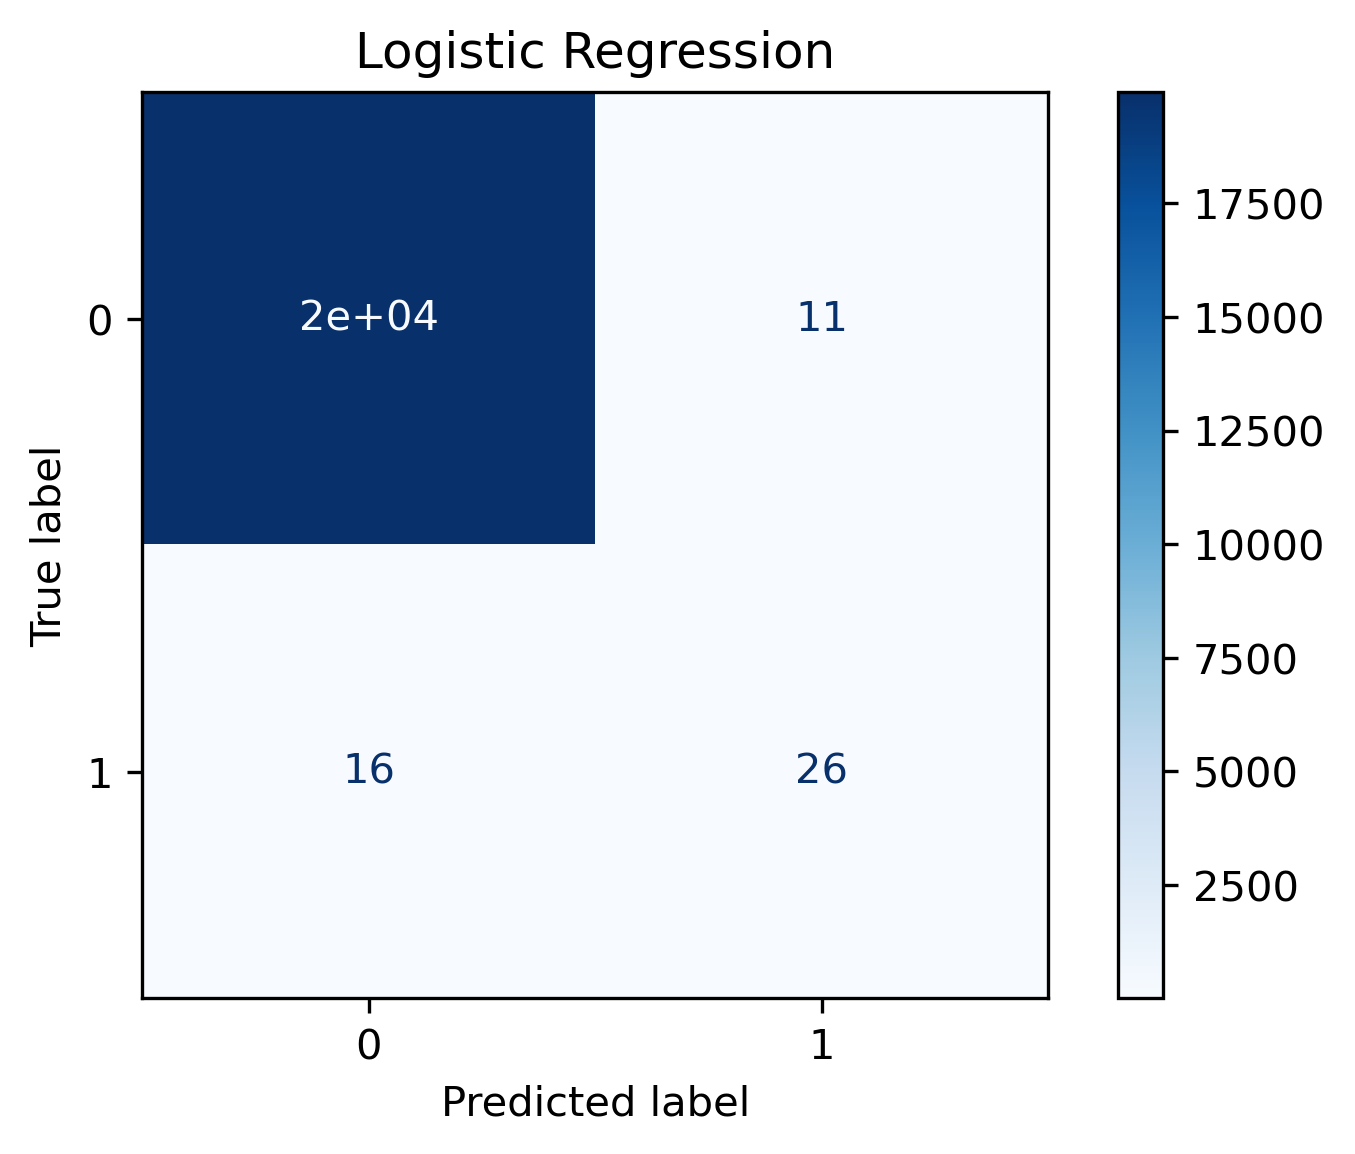
\includegraphics[width=\textwidth]{./images/reg_conf1.png}
    \label{fig:qqplotreszprice}
  \end{subfigure}
  \begin{subfigure}[b]{0.32\textwidth}
    \centering
    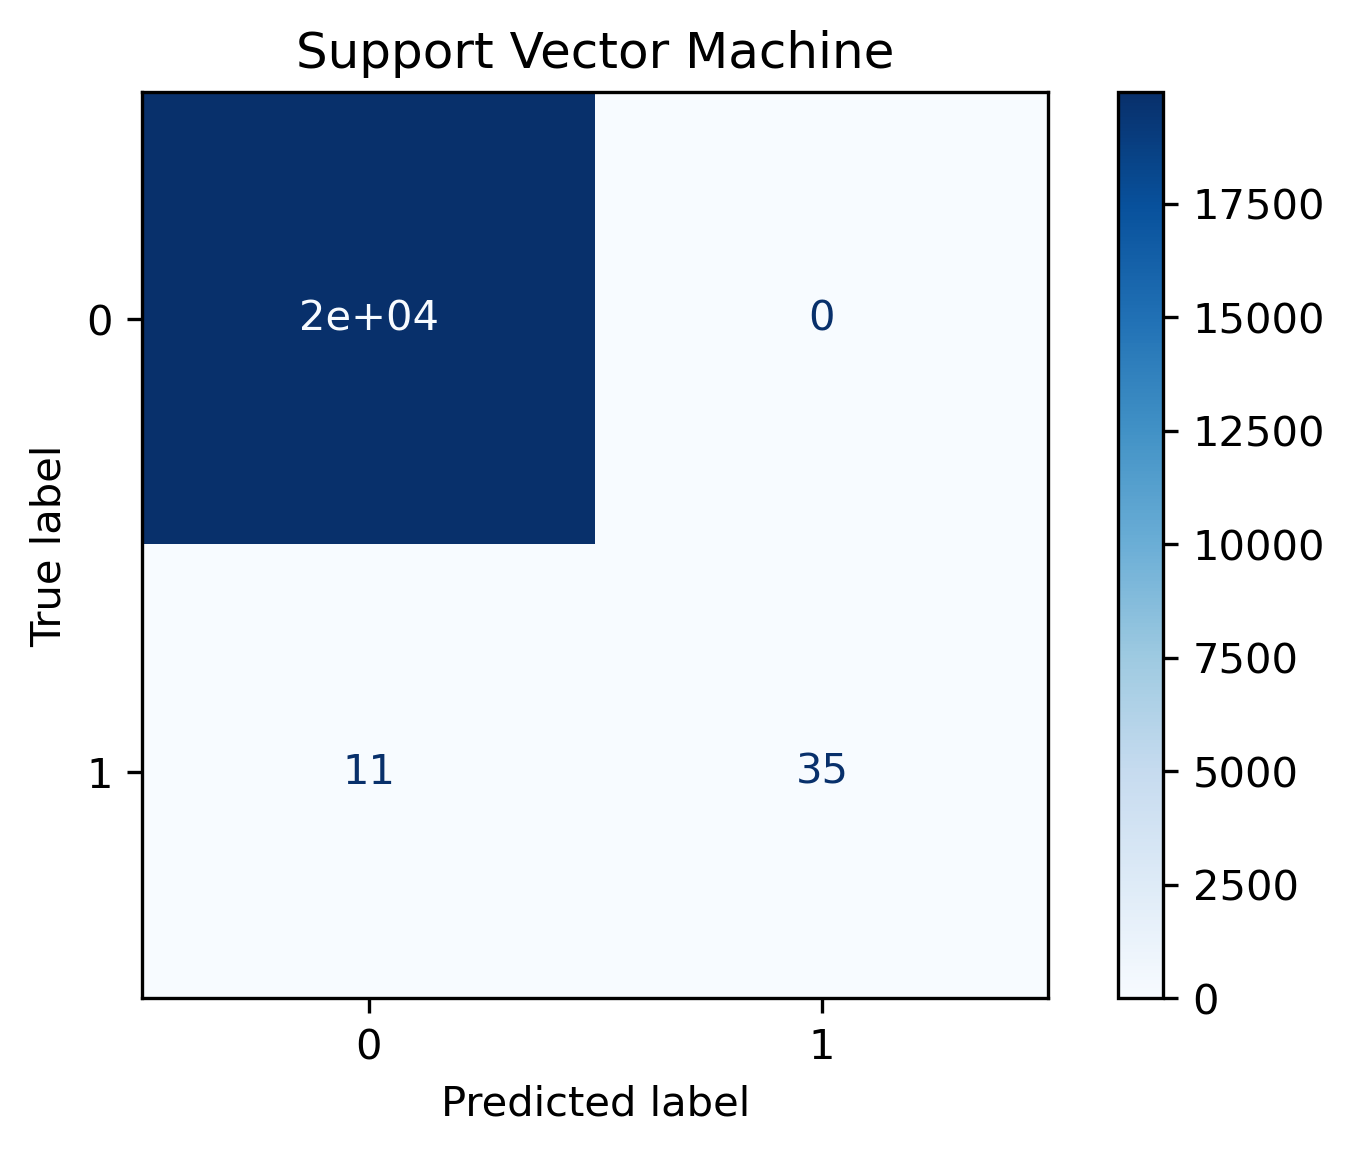
\includegraphics[width=\textwidth]{./images/svm_conf1.png}
    \label{fig:qqplotyyhatprice}
  \end{subfigure}
  \begin{subfigure}[b]{0.32\textwidth}
    \centering
    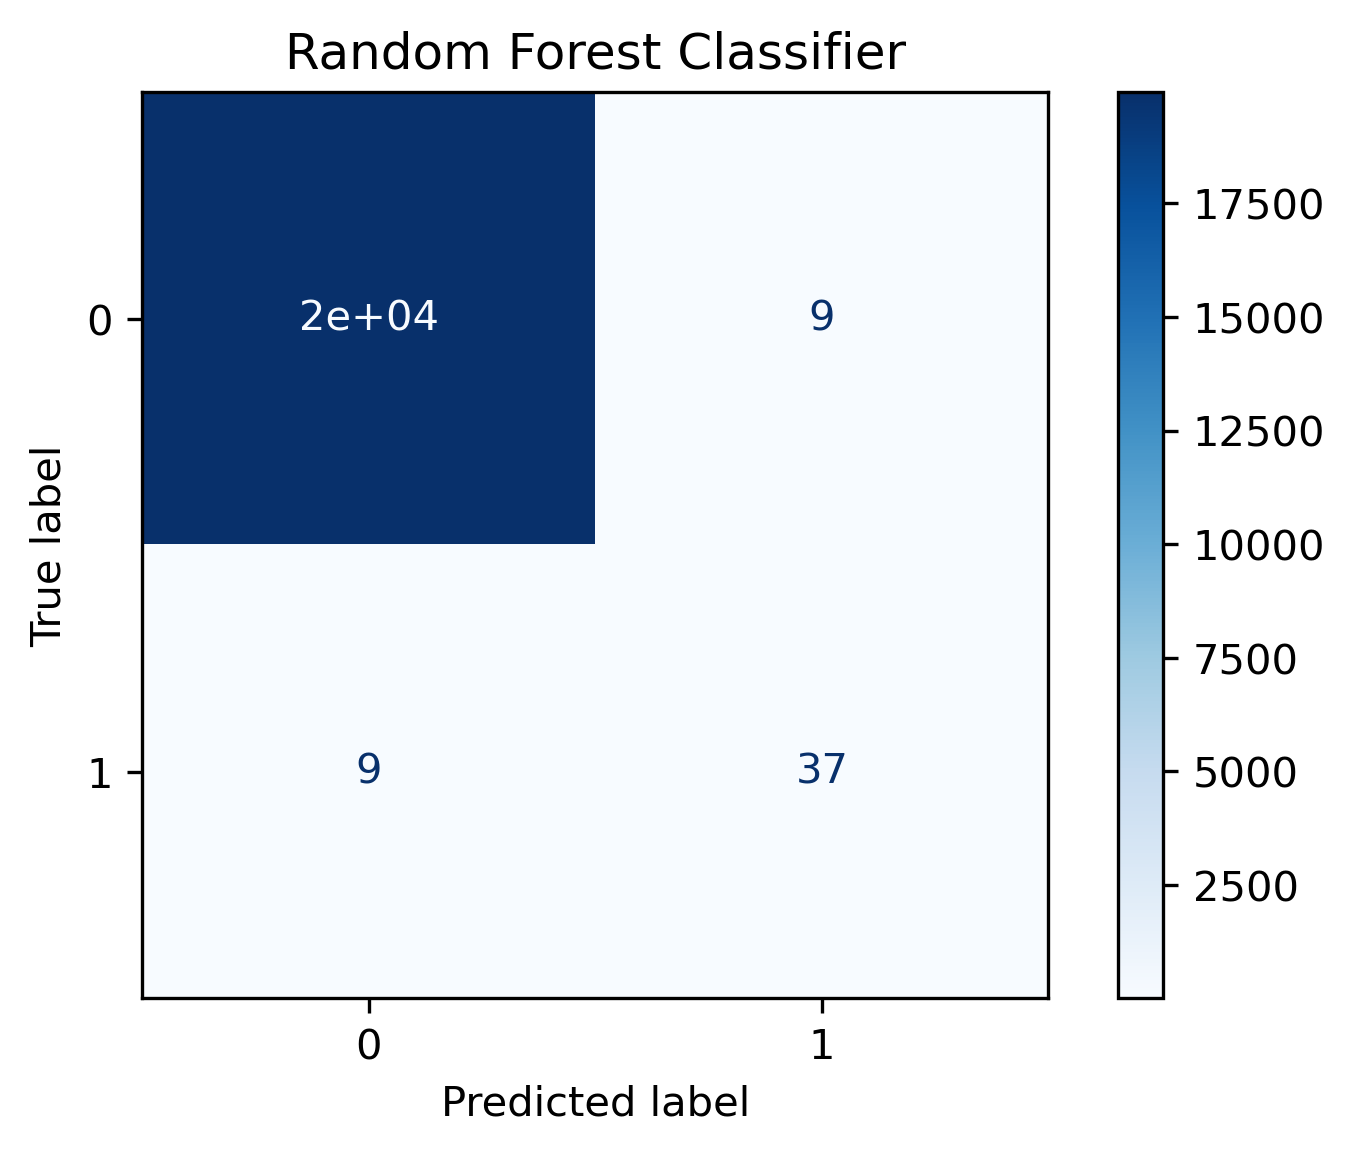
\includegraphics[width=\textwidth]{./images/rfc_conf1.png}
    \label{fig:scalelocationplotprice}
  \end{subfigure}
  \caption{Confusion matrices for logistic regression, SVM and Random Forest on test data}
  \label{fig:confusion1}
\end{figure}

\begin{table}[ht]
  \centering
  \caption{Accuracy, Precision, Recall and F1-Score for the 3 models}
  \label{tab:metrics1}
  \begin{tabular}{c|cccc}
    Model                    & Accuracy & Precision & Recall & F1-Score \\
    \hline
    Logistic Regression      & 0.9989   & 0.8000    & 0.6957 & 0.7442   \\
    Support Vector Machine   & 0.9994   & 1.000     & 0.7609 & 0.8642   \\
    Random Forest Classifier & 0.9991   & 0.8043    & 0.8043 & 0.8043   \\
  \end{tabular}
\end{table}

\subsection{Constructing a Deep Neural Network}

Secondly we construct a deep neural network and compare it to the methods previously presented.
The network has an input layer with 30 nodes, one for each feature. Then there are $d$ fully connected hidden layers, each consisting of $k$ neurons. A ReLU layer is put in between each two neighboring hidden layers. In the end, there is one output node, to which a sigmoid function is applied, to convert scores to probabilities. If the output is greater or equal to 0.5 we classify a case as fraud, otherwise as non-fraud.
There are some parameters that we need to set in advance:
\begin{enumerate}
  \item The number of hidden layers $d$.
  \item The number of nodes in each hidden layer $k$.
  \item The learning rate $LR$
  \item The batch size $b$
\end{enumerate}



\subsection{Summary}

\newpage
\addcontentsline{toc}{section}{Bibliography}
\renewcommand\refname{Bibliography}
\bibliographystyle{plainnat}
\bibliography{references}
\end{document}
